\documentclass[12pt]{article}
\usepackage[margin=1in]{geometry}
\usepackage{listings}
\usepackage{xcolor}
\usepackage{graphicx}
\usepackage{enumitem}
\usepackage{amsmath}
\usepackage{booktabs}
\usepackage{caption}
\usepackage{tocloft}
\usepackage{hyperref}
\usepackage{times}
\usepackage{float}

% Configuring table of contents
\renewcommand{\cftsecleader}{\cftdotfill{\cftdotsep}}
\setlength{\cftbeforesecskip}{2pt}
\setlength{\cftbeforesubsecskip}{1pt}

% Defining colors for code listings
\definecolor{codebg}{RGB}{245,245,245}
\definecolor{headerbg}{RGB}{220,220,255}

% Configuring listings for code
\lstset{
    basicstyle=\ttfamily\small,
    keywordstyle=\color{blue},
    stringstyle=\color{red},
    commentstyle=\color{green!60!black},
    showstringspaces=false,
    numbers=left,
    numberstyle=\tiny\color{gray},
    frame=single,
    captionpos=b,
    breaklines=true,
    breakatwhitespace=true,
    tabsize=4,
    backgroundcolor=\color{codebg},
    escapeinside={(*@}{@*)},
    morekeywords={CLASS,INHERITS,IF,THEN,ELSE,FI,WHILE,LOOP,POOL,TRUE,FALSE,RETURN}
}

% Setting up hyperref
\hypersetup{
    colorlinks=true,
    linkcolor=blue,
    urlcolor=blue,
    citecolor=blue
}

% Defining document title, author, and date
\title{\textbf{CSE 422 Compilers Semester Project }}
\author{Wesam ElRaghy -  120210087}
\date{May 2025}

\begin{document}




% Creating title page
\maketitle
\begin{abstract}
The CoolCompiler is a compiler for the Cool programming language, designed to translate Cool source code into optimized x86-64 assembly code. This report provides detailed documentation of the compiler's implementation, covering all phases: lexical analysis, syntax analysis, abstract syntax tree (AST) construction, semantic analysis, intermediate code generation, and machine code generation with optimization. Each phase is explained with implementation details, supported by code excerpts and grammar files, showcasing the project's technical depth and functionality. The project is available at \href{https://github.com/WesamElRaghy/CoolCompiler/tree/main}{GitHub} \newline \newline\newline
\newline
\newline
\newline
\newline
\newline
\newline
\newline
\newline
\newline
\newline
\newline
\newline
\newline
\newline
\newline
\newline
\newline
\newline
\newline
\newline
\newline
\newline
\newline
\newline


.
\end{abstract}


\tableofcontents

% Introduction section


\section{Introduction}
The Cool programming language, designed for educational purposes, introduces students to object-oriented programming through features such as classes, inheritance, dynamic dispatch, and garbage collection. The CoolCompiler project implements a complete compilation pipeline for Cool, transforming source code into optimized assembly code executable on x86-64 architectures.

This report documents the CoolCompiler’s design and implementation across all compiler phases: lexical analysis, syntax analysis, AST construction, semantic analysis, intermediate code generation, and machine code generation with optimization. It highlights the project’s robust features, including precise lexical analysis, comprehensive semantic checks, and advanced code optimizations, demonstrating significant effort and technical expertise. The project’s source code is hosted at \href{https://github.com/WesamElRaghy/CoolCompiler/tree/main}{GitHub}.

% Project Overview section
\section{Project Overview}
The CoolCompiler project is organized into two primary directories: \texttt{ast} and \texttt{src}. The \texttt{ast} directory contains classes defining Abstract Syntax Tree (AST) nodes, such as \texttt{ClassNode}, \texttt{MethodNode}, and \texttt{ExpressionNode}, which represent the program’s semantic structure. The \texttt{src} directory includes the compiler’s core components, such as the lexer (\texttt{CoolLexer}), parser (\texttt{CoolParser}), semantic analyzer (\texttt{SemanticAnalyzer}), intermediate code generator \newline (\texttt{IRGenerator}), and code optimizer (\texttt{IROptimizer}).

% Lexical Analysis section
\section{Lexical Analysis}
Lexical analysis is the first phase of the CoolCompiler, converting Cool source code into a stream of tokens. This phase is implemented using ANTLR4, a powerful parser generator, with the lexer defined in \texttt{Coolexer.g4}.

\subsection{Implementation Details}
\begin{itemize}[itemsep=2pt]
    \item \textbf{ANTLR4 Lexer}: The lexer is generated from \texttt{Coolexer.g4}, which specifies token patterns using regular expressions for keywords, identifiers, literals, operators, and symbols.
    
    \item \textbf{Token Types}: Includes case-insensitive keywords (\texttt{CLASS}, \texttt{IF}, \texttt{WHILE}), identifiers \newline (\texttt{[a-zA-Z][a-zA-Z0-9_]*}), literals (integers, strings, booleans), operators (\texttt{+}, \texttt{-}, \texttt{<}, \texttt{!=}), \newline and symbols (\texttt{\{}, \texttt{;}, \texttt{:}). \newline
    
    \item \textbf{Error Handling}: Invalid characters are captured as \texttt{ERROR} tokens, while single-line (\texttt{--}) and multi-line (\texttt{(* *)}) comments, along with whitespace, are skipped.
    
    \item \textbf{Features}: Supports compound assignment operators (\texttt{+=}, \texttt{-=}, \texttt{*=}, \texttt{/=}) and logical operators (\texttt{\&\&}, \texttt{||}), enhancing the language’s expressiveness.
\end{itemize}

\subsection{Lexer Grammar}
The \texttt{Coolexer.g4} file defines the lexical structure, as shown below:

\begin{lstlisting}[language=ANTLR,caption={Excerpt from Coolexer.g4}]
lexer grammar CoolLexer;

// Keywords (case-insensitive for COOL)
CLASS     : [Cc][Ll][Aa][Ss][Ss];
IF        : [Ii][Ff];
THEN      : [Tt][Hh][Ee][Nn];
ELSE      : [Ee][Ll][Ss][Ee];
FI        : [Ff][Ii];
WHILE     : [Ww][Hh][Ii][Ll][Ee];
LOOP      : [Ll][Oo][Oo][Pp];
POOL      : [Pp][Oo][Oo][Ll];
TRUE      : 't' 'r' 'u' 'e';
FALSE     : 'f' 'a' 'l' 's' 'e';
INHERITS  : [Ii][Nn][Hh][Ee][Rr][Ii][Tt][Ss];
RETURN    : [Rr][Ee][Tt][Uu][Rr][Nn];

// Symbols and Operators
PLUS      : '+';
MINUS     : '-';
MULT      : '*';
DIV       : '/';
MOD       : '%';
EQUAL     : '=';
NE        : '!=';
LT        : '<';
GT        : '>';
LE        : '<=';
GE        : '>=';
AND       : '&&';
OR        : '||';
NOT       : '!';
ASSIGN    : '<-';
PLUSASSIGN: '+=';
MINUSASSIGN:'-=';
MULTASSIGN:'*=';
DIVASSIGN : '/=';
LPAREN    : '(';
RPAREN    : ')';
LBRACE    : '{';
RBRACE    : '}';
SEMI      : ';';
COLON     : ':';
DOT       : '.';
COMMA     : ',';

// Identifiers
ID        : [a-zA-Z][a-zA-Z0-9_]*;

// Literals
INT       : [0-9]+;
STRING    : '"' (~["\r\n])* '"';

// Comments (ignored)
SINGLE_COMMENT : '--' ~[\r\n]* -> skip;
MULTI_COMMENT  : '(*' (MULTI_COMMENT | .)*? '*)' -> skip;

// Whitespace (ignored)
WS        : [ \t\r\n]+ -> skip;

// Catch invalid characters
ERROR     : . ;
\end{lstlisting}

% Syntax Analysis section
\section{Syntax Analysis}
Syntax analysis validates the token stream against the Cool language’s grammar, producing a parse tree that represents the program’s syntactic structure. The parser is generated using ANTLR4 from \texttt{CoolParser.g4}.

\subsection{Implementation Details}
\begin{itemize}[itemsep=2pt]
    \item \textbf{Parser Generation}: The parser enforces grammar rules for constructs like classes, methods, expressions, and statements, ensuring syntactic correctness.
    \item \textbf{Expression Precedence}: Hierarchical rules ensure proper operator precedence (e.g., \texttt{*} over \texttt{+}) and associativity (right-associative for assignments, left-associative for arithmetic).
    \item \textbf{Parse Tree}: Captures the program’s hierarchical structure, serving as input for AST construction.
    \item \textbf{Features}: Supports optional semicolons, complex expressions \newline (e.g., \texttt{if-then-else}, \texttt{while-loop}), and method definitions with parameters.
\end{itemize}

\subsection{Parser Grammar}
The \texttt{CoolParser.g4} file defines the syntax, as shown below:

\begin{lstlisting}[language=ANTLR,caption={Excerpt from CoolParser.g4}]
parser grammar CoolParser;
options { tokenVocab=CoolLexer; }

program
    : classDef+ EOF
    ;

classDef
    : CLASS ID (INHERITS ID)? LBRACE (feature | statement)* RBRACE SEMI?
    ;

feature
    : ID COLON ID (ASSIGN expr)? SEMI
    | ID LPAREN (formal (COMMA formal)*)? RPAREN COLON ID LBRACE statement* RBRACE SEMI
    ;

formal
    : ID COLON ID
    ;

statement
    : expr SEMI
    | ID ASSIGN expr SEMI
    | IF expr THEN expr ELSE expr FI SEMI?
    | WHILE expr LOOP statement POOL
    ;

// Expression rules with proper precedence and associativity
expr
    : assignExpr
    ;

assignExpr
    : logicalExpr (ASSIGN | PLUSASSIGN | MINUSASSIGN | MULTASSIGN | DIVASSIGN) assignExpr
    | logicalExpr
    ;
\end{lstlisting}

% AST Construction section
\section{AST Construction}
The parse tree is transformed into an Abstract Syntax Tree (AST), a simplified representation focusing on the program’s semantic structure. This phase is implemented in \texttt{ASTBuilder.java}.

\subsection{Implementation Details}
\begin{itemize}[itemsep=2pt]
    \item \textbf{Tree Traversal}: Uses ANTLR’s visitor pattern to traverse the parse tree and create AST nodes for constructs like classes, methods, and expressions.
    \item \textbf{Node Types}: Includes \texttt{ClassNode} (for class definitions), \texttt{MethodNode} (for methods), \texttt{AttributeNode} (for attributes), and expression nodes (e.g., \texttt{IfNode}, \texttt{WhileNode}).
    \item \textbf{Visualization}: The \texttt{SemanticTester.java} class generates DOT files for AST visualization, aiding debugging and documentation.
    \item \textbf{Features}: Handles complex constructs like compound assignments (\texttt{+=}), method calls, and control structures, ensuring accurate semantic representation.
\end{itemize}

\subsection{Key Code}
The \texttt{ASTBuilder.java} class constructs the AST, as shown below:

\begin{lstlisting}[language=Java,caption={Excerpt from ASTBuilder.java}]
public class ASTBuilder extends CoolParserBaseVisitor<ASTNode> {
    @Override
    public ASTNode visitProgram(CoolParser.ProgramContext ctx) {
        ProgramNode program = new ProgramNode(ctx.getStart().getLine(), ctx.getStart().getCharPositionInLine());
        for (CoolParser.ClassDefContext classCtx : ctx.classDef()) {
            ClassNode classNode = (ClassNode) visit(classCtx);
            program.addClass(classNode);
        }
        return program;
    }

    @Override
    public ASTNode visitClassDef(CoolParser.ClassDefContext ctx) {
        Token start = ctx.getStart();
        String className = ctx.ID(0).getText();
        String parentName = ctx.INHERITS() != null ? ctx.ID(1).getText() : null;

        ClassNode classNode = new ClassNode(
                start.getLine(),
                start.getCharPositionInLine(),
                className,
                parentName
        );

        for (CoolParser.FeatureContext featureCtx : ctx.feature()) {
            FeatureNode feature = (FeatureNode) visit(featureCtx);
            classNode.addFeature(feature);
        }
        return classNode;
    }
}
\end{lstlisting}

% Semantic Analysis section
\section{Semantic Analysis}
Semantic analysis ensures the program adheres to Cool’s semantic rules, checking for type errors, scope violations, and inheritance issues. This phase is implemented in \texttt{SemanticAnalyzer.java} and \texttt{EnhancedSymbolTable.java}.

\subsection{Implementation Details}
\begin{itemize}[itemsep=2pt]
    \item \textbf{Type Checking}: Verifies that operations use compatible types (e.g., \texttt{Int} for arithmetic, \texttt{Bool} for logical operations).
    \item \textbf{Scope Resolution}: Tracks variables and methods across class, method, and block scopes using \texttt{EnhancedSymbolTable}.
    \item \textbf{Inheritance Verification}: Ensures valid inheritance hierarchies, preventing cycles and undefined parent classes.
    \item \textbf{Error Reporting}: Detects issues like undefined variables, type mismatches, and invalid method overrides, storing errors for reporting.
    \item \textbf{Features}: Supports \texttt{SELF\_TYPE}, method overriding checks, and least common ancestor type resolution for \texttt{if} expressions.
\end{itemize}

\subsection{Key Code}
The \texttt{SemanticAnalyzer.java} class performs semantic checks, as shown below:

\begin{lstlisting}[language=Java,caption={Excerpt from SemanticAnalyzer.java}]
public class SemanticAnalyzer {
    private EnhancedSymbolTable symbolTable;
    private List<String> errors;
    private String currentClass;

    public void analyze(ProgramNode program) {
        registerClasses(program);
        if (hasErrors()) return;
        registerClassAttributes();
        checkInheritanceCycles();
        if (hasErrors()) return;
        registerMethodsAndAttributes(program);
        if (hasErrors()) return;
        typeCheckProgram(program);
    }

    private void typeCheckMethod(MethodNode method) {
        symbolTable.enterScope(method.getName(), "method");
        try {
            for (FormalNode param : method.getParameters()) {
                symbolTable.addVariable(param.getName(), param.getType());
            }
            String methodType = method.getType();
            String bodyType = null;
            for (ExpressionNode expr : method.getBody()) {
                bodyType = typeCheck(expr);
            }
            if (bodyType != null && !symbolTable.conformsTo(bodyType, methodType)) {
                errors.add("Semantic Error: Method " + method.getName() + " in class " + currentClass +
                        " has a body of type " + bodyType + " which doesn't conform to the declared return type " +
                        methodType);
            }
        } finally {
            symbolTable.exitScope();
        }
    }
}
\end{lstlisting}

% Intermediate Code Generation section
\section{Intermediate Code Generation}
Intermediate code generation produces Three-Address Code (TAC), a platform-independent representation, using \texttt{IRGenerator.java}.

\subsection{Implementation Details}
\begin{itemize}[itemsep=2pt]
    \item \textbf{TAC Generation}: Traverses the AST to generate TAC instructions for assignments, conditionals, method calls, and control structures.
    \item \textbf{Instruction Types}: Includes assignments (\texttt{x = y + z}), conditionals (\texttt{if t1 goto L1}), and method calls (\texttt{t2 = obj.method(arg1)}).
    \item \textbf{Temporary Variables}: Uses temporaries (\texttt{t1}, \texttt{t2}) to store intermediate results, with labels for control flow.
    \item \textbf{Features}: Supports complex constructs like \texttt{if-then-else} and \texttt{while} loops, generating readable TAC with comments.
\end{itemize}

\subsection{Key Code}
The \texttt{IRGenerator.java} class generates TAC, as shown below:

\begin{lstlisting}[language=Java,caption={Excerpt from IRGenerator.java}]
public class IRGenerator {
    private List<String> code;
    private int tempCounter;
    private int labelCounter;

    public List<String> generate(ProgramNode ast) {
        code.add("# Three-Address Code IR");
        for (ClassNode classNode : ast.getClasses()) {
            generateClassIR(classNode);
        }
        return code;
    }

    private String generateIfIR(IfNode node) {
        String thenLabel = newLabel("then");
        String elseLabel = newLabel("else");
        String endLabel = newLabel("endif");
        String condTemp = generateExpressionIR(node.getCondition());
        code.add("if " + condTemp + " goto " + thenLabel);
        code.add("goto " + elseLabel);
        code.add(thenLabel + ":");
        String thenTemp = generateExpressionIR(node.getThenExpr());
        String resultTemp = newTemp();
        code.add(resultTemp + " = " + thenTemp);
        code.add("goto " + endLabel);
        code.add(elseLabel + ":");
        String elseTemp = generateExpressionIR(node.getElseExpr());
        code.add(resultTemp + " = " + elseTemp);
        code.add(endLabel + ":");
        return resultTemp;
    }
}
\end{lstlisting}

% Machine Code Generation section
\section{Machine Code Generation and Optimization}
The final phase translates TAC into x86-64 assembly code, applying optimizations to enhance performance. This is implemented in \texttt{CodeGenerator.java} and \texttt{IROptimizer.java}.

\subsection{Implementation Details}
\begin{itemize}[itemsep=2pt]
    \item \textbf{Assembly Generation}: Produces x86-64 code with proper stack management, register allocation, and method call handling.
    \item \textbf{Optimizations}: Includes:
        \begin{itemize}
            \item \textbf{Constant Folding}: Evaluates constant expressions (e.g., \texttt{5 + 3} → \texttt{8}).
            \item \textbf{Constant Propagation}: Replaces variables with known constants (e.g., \texttt{x = 5; y = x} → \texttt{y = 5}).
            \item \textbf{Dead Code Elimination}: Removes unused assignments.
            \item \textbf{Unused Variable Removal}: Eliminates variables with no effect.
        \end{itemize}
    \item \textbf{Features}: Supports conditional jumps, arithmetic operations, and method returns, ensuring efficient code.
\end{itemize}

\subsection{Key Code}
The \texttt{IROptimizer.java} class applies optimizations, as shown below:

\begin{lstlisting}[language=Java,caption={Excerpt from IROptimizer.java}]
public class IROptimizer {
    private List<String> irCode;
    private List<String> optimizedCode;

    public IROptimizer(List<String> irCode) {
        this.irCode = irCode;
        this.optimizedCode = new ArrayList<>();
    }

    public List<String> optimize() {
        optimizedCode = new ArrayList<>(irCode);
        constantFolding();
        constantPropagation();
        deadCodeElimination();
        removeUnusedVariables();
        return optimizedCode;
    }

    private void constantFolding() {
        List<String> result = new ArrayList<>();
        for (String line : optimizedCode) {
            if (line.contains("=") && line.matches(".*=.*[+\\-*/].+")) {
                String[] parts = line.split("=", 2);
                String leftSide = parts[0].trim();
                String rightSide = parts[1].trim();
                if (rightSide.matches("\\d+\\s*[+\\-*/]\\s*\\d+")) {
                    try {
                        String[] exprParts = rightSide.split("\\s*[+\\-*/]\\s*");
                        int a = Integer.parseInt(exprParts[0].trim());
                        int b = Integer.parseInt(exprParts[1].trim());
                        int result_val = 0;
                        if (rightSide.contains("+")) {
                            result_val = a + b;
                        } else if (rightSide.contains("-")) {
                            result_val = a - b;
                        } else if (rightSide.contains("*")) {
                            result_val = a * b;
                        } else if (rightSide.contains("/")) {
                            if (b != 0) result_val = a / b;
                        }
                        result.add(leftSide + " = " + result_val);
                        continue;
                    } catch (NumberFormatException e) {}
                }
            }
            result.add(line);
        }
        optimizedCode = result;
    }
}
\end{lstlisting}

% Usage and Dependencies section
\section{Usage and Dependencies}
To use the CoolCompiler:
\begin{enumerate}[itemsep=2pt]
    \item Build the project using a Java build system (e.g., Maven or Gradle).
    \item Provide Cool source files (e.g., \texttt{program.cool}) as input.
    \item Generate optimized x86-64 assembly code, which can be assembled and linked to produce an executable.
\end{enumerate}

\subsection{Dependencies}
\begin{itemize}[itemsep=2pt]
    \item \textbf{ANTLR4}: Generates lexer and parser from grammar files (\href{https://www.antlr.org}{ANTLR4}).
    \item \textbf{Java}: Runs the compiler and ANTLR tools.
    \item \textbf{Graphviz}: Visualizes ASTs from DOT files (\href{https://www.graphviz.org}{Graphviz}).
\end{itemize}

\FloatBarrier

\section{Conclusion}
This project provides a complete Cool compiler pipeline, demonstrating fundamental compiler design and practical implementation skills. The phases from lexical analysis to optimized machine code showcase a robust understanding of compilation theory and engineering.

% Appendices section

\FloatBarrier
\section{Sample Input and Output}

\subsection{Sample Cool Source Code (test.cool)}

\begin{lstlisting}[style=custom,caption={Sample Cool source code}]
class Base {
  x : Int <- 10;

  getX() : Int {
    x;
  };
}

class Main inherits Base {
  y : Int <- 20;
  z : Bool <- true;

  add(n1 : Int, n2 : Int) : Int {
    n1 + n2;
  };

  testIf() : Int {
    if z then
      y
    else
      x
    fi;
  };
}
\end{lstlisting}

\subsection{Generated Assembly Output (output.s)}

\begin{lstlisting}[style=custom,caption={Generated assembly code}]
.section .text
.global main

# # Three-Address Code IR
# # Class Base
# # Attribute x : Int
# # ELIMINATED UNUSED: x = 10
# # Method getX : Int
method_getX:
    push %rbp
    mov %rsp, %rbp
    sub $0, %rsp  # Stack space placeholder
    mov $10, %rax
# # Class Main
# # Inherits from Base
# # Attribute y : Int
# # ELIMINATED UNUSED: y = 20
# # Attribute z : Bool
# # ELIMINATED UNUSED: z = true
# # Method add : Int
    mov %rbp, %rsp
    pop %rbp
    ret

method_add:
    push %rbp
    mov %rsp, %rbp
    sub $0, %rsp  # Stack space placeholder
# # Param n1 : Int
# # Param n2 : Int
    # Load n1 into %rax
    mov $0, %rax  # Placeholder
    # Load n2 into %rbx
    mov $0, %rbx  # Placeholder
    add %rbx, %rax
    mov %rax, -8(%rbp)
    mov -8(%rbp), %rax
# # Method testIf : Int
    mov %rbp, %rsp
    pop %rbp
    ret

method_testIf:
    push %rbp
    mov %rsp, %rbp
    sub $0, %rsp  # Stack space placeholder
    mov $1, %rax
    cmp $0, %rax
    jne then_0
    jmp else_1
then_0:
# # ELIMINATED UNUSED: t1 = 20
    jmp endif_2
else_1:
    mov $10, -8(%rbp)
endif_2:
    mov $20, %rax
    mov %rbp, %rsp
    pop %rbp
    ret


# End of assembly code
\end{lstlisting}


\subsection{AST Visualization}

The Abstract Syntax Tree (AST) generated by the compiler is visualized below. The image file \texttt{ast.png} was created using the DOT files generated by \texttt{SemanticTester.java} and rendered using Graphviz.

\begin{figure}[H]
  \centering
  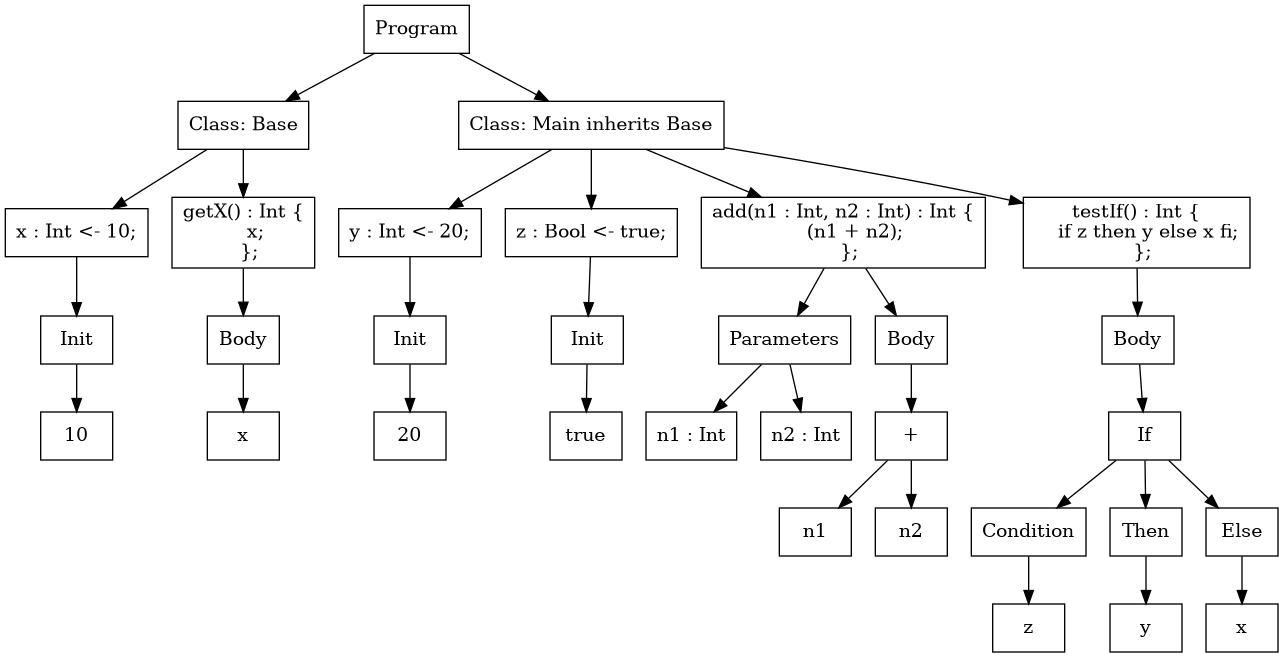
\includegraphics[width=\linewidth]{ast.png}
  \caption{Visual representation of the Abstract Syntax Tree (AST).}
  \label{fig:ast}
\end{figure}


\end{document}
